\chapter{BumbleBee}
\label{bumblebee}
\index{BumbleBee%
@\emph{BumbleBee}}%

Because one of Honeycomb's goals is to decouple the user track gathering mechanism from the location estimation mechanisms, we needed a tool with which to gather user tracks in order to prove Honeycomb's effectiveness. Fortunately, in a previous, unpublished project, the author of this paper co-wrote precisely that tool, called BumbleBee. BumbleBee's only purpose is to provide a viable user track gathering tool in order to feed user track data into a location estimation system. Here, we describe BumbleBee in more detail.


\section{Infrastructure}
\index{Infrastructure@\emph{Infrastructure}}%

Bumblebees major contribution is its novel infrastructure (Figure \ref{bumblebeearch}), in which there exists a Wi-Fi network host, the “Gatekeeper”, at the store entrance. As mobile devices, the “bumblebees”, enter the store, they connect to the Gatekeeper and request work. The Gatekeeper provides the bumblebee the BSSIDs addresses of N Wi-Fi access points located throughout the store, where N is the number of different access points from which the Gatekeeper wants signal strength measurements. When the bumblebee leaves the store, and detects that it is once again in range of the Gatekeeper, it makes another connection to the Gatekeeper and hands over its data. Employing the Gatekeeper as data sink allows the bumblebee to drop its collected data off and free its memory. The Gatekeeper can then aggregate the data and deliver it to the site specific location estimator, allowing both the bumblebees and the Gatekeeper to be agnostic of the location estimation method.

We believe that the real novelty of BumbleBee lies in the introduction of the Gatekeeper. Serving dual roles, both as distributor of work and as data sink, the Gatekeeper is the driving force in the system. Because bumblebees are mobile and the Gatekeeper is not, employing the Gatekeeper as the distributor of work allows for site specific configurations, and allows the bumblebee to easily move into and out of various deployments without any a priori knowledge of the site specific deployment save for the identity of the Gatekeeper.


\begin{figure}[htb] % Imported eps example.
	\begin{center}
		\ 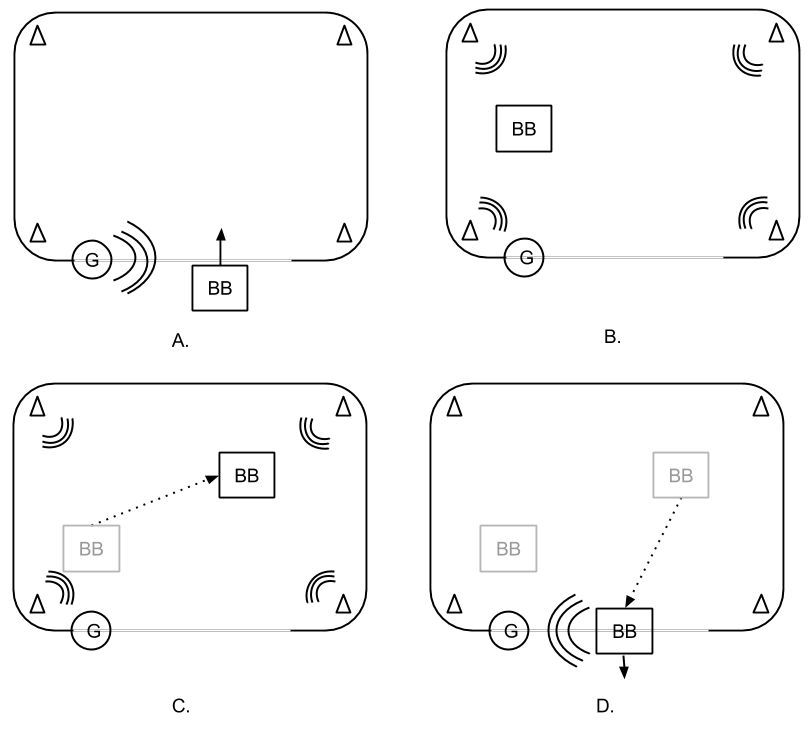
\includegraphics[width=4in,height=3in]{BumbleBeeExample.png}
		\caption{BumbleBee Architecture}
		\label{bumblebeearch}
	\end{center}
\end{figure}


\section{Implementation}
\index{Implementation@\emph{Implementation}}%


\subsection{The Gatekeeper}
\index{Gatekeeper@\emph{Gatekeeper}}%

The gatekeeper is implemented in the Python programming language so that it can remain relatively platform independent. It is comprised of three main components: the gatekeeper network service, a GUI, and a plugin interface to allow extending the systems functionality. We have implemented plugins for saving/restoring results to/from disk, graphing received signal strength from all BSSIDs across time, logging, and exporting results to a portable format for use outside BumbleBee. As part of the Honeycomb project, we also implemented a Gatekeeper plugin for uploading user tracks to the Honeycomb API. The Gatekeeper server listens on a fixed TCP port (0xb33) for requests from clients through remote procedure calls (via Python’s SimpleXMLRPCServer). Information exchange with the bumblebees is done in JSON data format. The gatekeeper administrator configures the BSSIDs addresses and minimum polling interval.


\subsection{The Bumblebee}
\index{The Bumblebee@\emph{The Bumblebee}}%

The bumblebee component is implemented as an Android application written in the Java programming language. The application performs three main tasks: automatic network detection of the Gatekeeper, negotiation with the Gatekeeper, and data collection related activities. These operations require no user interaction and thus we consider this application unobtrusive. As part of the data collection process the bumblebee application will wake up on the negotiated time interval, observe broadcasting wireless networks, and collect and store signal strength values for all requested BSSIDs. It then stamps the collected data with the offset from the time it collected the work from the Gatekeeper and returns to sleep. The periodic waking process is also used to rediscover the Gatekeeper. When the Gatekeeper is rediscovered the application once again negotiates a connection, but this time instead of accepting work it submits the collected data. The data is then discarded from the mobile device.


\subsection{Communication Mechanism}
\index{Communication Mechanism@\emph{Communication Mechanism}}%


The bumblebee mobile device communication model is shown in Figure \ref{bumblebestatediagram}. The initial state of the bumblebee is ‘Sleeping / Inactive’ (with respect to BumbleBee activities). Upon discovery of the Gatekeeper the application enters the ‘Handshake’ state. In this state the application may choose to not accept the requested task, in which case it moves back to the ‘Sleeping / Inactive’ state. If work is accepted then the application moves into the ‘Data Collection’ state. The data collection process was described in the previous section. The handshake process is described below. When the bumblebee once again discovers the Gatekeeper is once again enters the ‘Handshake’ state, but this time it transmits the collected data to the Gatekeeper. Once this is completed, the bumblebee moves back into the ‘Sleeping / Inactive’ state.

The handshake between Gatekeeper and a bumblebee client happens within the context of a single connection-oriented session and involves a simple two-way handshake. The handshake happens after the bumblebee discovers the Gatekeeper and involves either the requesting of a new data collection information or the submission of collected data. In both cases the bumblebee initially transmits its unique ID to the Gatekeeper. This provides the Gatekeeper an opportunity to perform validation of the ID (perhaps to reference a user database or possibly black/white list of IDs). Assuming the ID is validated, and the client is making a request, a response is sent listing the BSSIDs to monitor, the maximum acceptable interval between samples, and the Gatekeeper’s current timestamp. The bumblebee is now in the ‘Data Collection’ state as described above. If the client is unable to support the request it silently drops the request and transitions back to the ‘Sleeping / Inactive’ state.

If the bumblebee successfully transitioned to the ‘Data Collection’ state and the Gatekeeper is once again discovered, the handshake process again takes place. After validation the bumblebee then transmits an overall status, the original request timestamp, and the series of collected timestamped signal strength values for all BSSIDs. Regardless of the status of the request the bumblebee moves to the ‘Sleeping / Inactive’ state. The Gatekeeper will store the request, regardless of status, for later analysis. In our case, this analysis actually occurs on Honeycomb hardware.


\begin{figure}[htb] % Imported eps example.
	\begin{center}
		\ 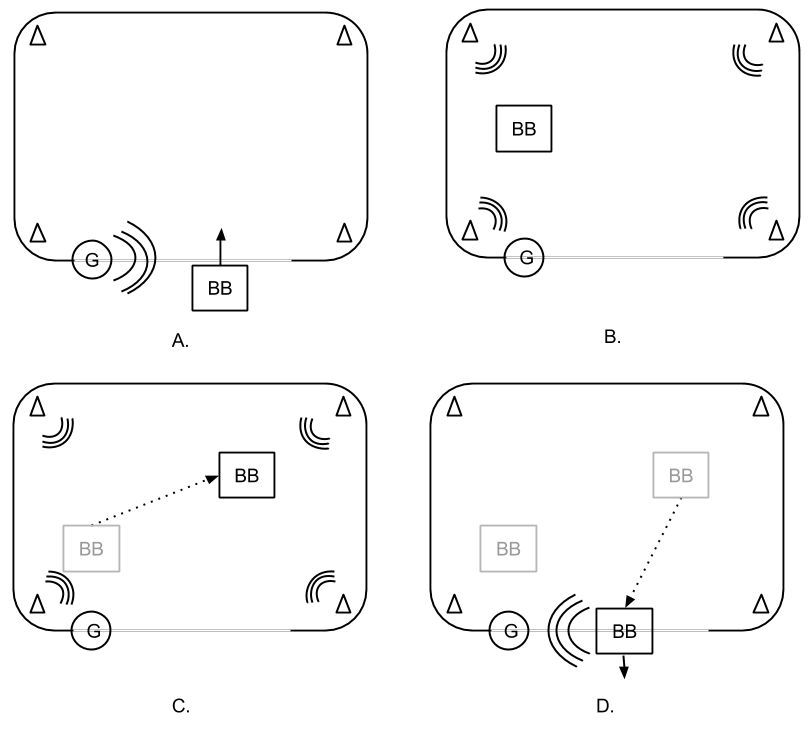
\includegraphics[width=4in,height=3in]{BumbleBeeExample.png}
		\caption{BumbleBee State Diagram}
		\label{bumblebestatediagram}
	\end{center}
\end{figure}
